\chapter{Learning Theory (20 pages)}
\label{learning-theory}

\section{Learning}

\section{Acquisition}

\section{Dynamics}

\section{Modeling}

The relationship between the discrete-time LRP scheme and its continuous-time solution is analogous to the difference between solution methods to an ordinary differential equation. The discrete-time version corresponds to Euler's method with step size $h=1$. Obviously, generations are not perfectly separated, nor are the perfectly overlapping. This means that the truth of things lies somewhere in between. We can either have the step size be a parameter that is fit in any given analysis, or we can adopt one functional form or the other and try to establish an error bound between the two.


Given an input sentence $s$, the learner selects a grammar $G_i$ with probability $p_i$:


\begin{equation}
 \mbox{If $G_i \rightarrow s$ then }
\left\{
	\begin{array}{ll}
		p_i'  = p_i + \gamma (1-p_i)\\
		p_j'  = (1-\gamma)p_j & \mbox{for} j \neq i
	\end{array}
\right.
\end{equation}

\begin{equation}
 \mbox{If $G_i \nrightarrow s$ then }
\left\{
	\begin{array}{ll}
		p_i'  = (1-\gamma ) p_i \\
		p_j'  = \frac{\gamma}{N - 1} + (1-\gamma)p_j & \mbox{for} j \neq i
	\end{array}
\right.
\end{equation}


\begin{equation}
     \frac{q_t}{p_t} = \left( \frac{\beta}{\alpha} \right)^t\frac{q_0}{p_0}
\end{equation}

"it is imperative that the learner punish grammars that fail to analyze incoming sentences. A special case of the algorithm $L (L')$ can be called a \emph{tolerant} learner, in which if a grammar succeeds in analyzing a sentences, it is rewarded; otherwise nothing happens. A tolerant learner corresponds to the \emph{Linear-Interaction} scheme (Atkinson et al. 1965), which has quite different stochastic properties, e.g. convergence is not always guaranteed." Yang 1999 p.14

Linear Reward-Inaction schema is known to be e-optimal \citep{narendra2012}

I'm working with a differential equation that is a logistic growth function with a carrying capacity and a varying growth rate, where $p, \alpha, \beta \in [0,1]$.

$\frac{dp}{dt} = p(1-p)\frac{\beta - \alpha}{(1-p)\alpha + p\beta}$

 The parameters $\alpha$ and $\beta$ determine the sign of the growth rate. If $\beta > \alpha$ then the growth rate is positive, if $\beta < \alpha$ then the growth rate is negative.

Integrating and taking antilogarithms we get the following, where $K$ comes from a constant of integration. 
 
 $\frac{p^\alpha}{(1-p)^\beta} = Ke^{(\beta - \alpha)t}$

Assuming that the $p = p_0$ at $t = 0$.

$K = \frac{p_0^\alpha}{(1-p_0)^\beta}$

I'm not sure how to use this to find a particular solution for $p$. In particular, I'm not sure how to deal with the exponents. Is there a way to solve for $p$? 

One potential route to take, would be to simplify the denominator in the growth rate of the original equation and consider the two simplified equations.

$\frac{dp}{dt} = p(1-p)\frac{\beta - \alpha}{\alpha}$

$\frac{dp}{dt} = p(1-p)\frac{\beta - \alpha}{\beta}$

with particular solutions where $K =\frac{p_0}{(1-p_0)}$

$p = \frac{Ke^{\frac{\beta}{\alpha}t}}{Ke^{\frac{\beta}{\alpha}t} + e^t}$

$p = \frac{Ke^t}{Ke^t + e^{\frac{\alpha}{\beta}t}}$

If $\beta > \alpha$ then the growth rate for the first simplified equation is always greater than the second simplified equation, and the solution to the original equation will be somewhere in between these two. Is there a straightforward way to interpolate between these two solutions?


The analysis presented in the previous section suggests that pragmatic pressures can lead to the increase in the use of a postverbal negator. The question is then why this increase so often leads to the loss of the preverbal negator. If, at some point, the postverbal negator comes to be negative in its own right, then this clearly impinges on the process of acquisition. Learners are faced with the problem of determining what exactly expresses negation. Here we examine how use and acquisition might allow for the transition from preverbal negation to postverbal negation. We consider whether the two mechanisms can independently bring about the change, or whether they must act in concert to destabilize the current system of negation.

At the heart of this question is the amount of evidence that a given element expresses negation. At the beginning of the change clearly only the preverbal negator does so. The postverbal reinforcer only emphasizes this negation. Eventually though, the evidence weighs in favor of the postverbal negator alone being the expression of negation. \cite{wallage2008} characterizes this transition in morphosyntactic terms as the loss of a [+NEG] feature on the preverbal negator, along with the concomitant introduction of a [+NEG] feature on the postverbal negator. This then allows for the loss of the preverbal negator given that the negative feature can be found elsewhere in the sentence.

We can formulate the effect of various amounts of evidence in terms of Yang's \citeyearpar{yang:2002} variational model. First, let there be two grammars, $G_{ne}$ and $G_{not}$, that represent the location of the abstract feature at \emph{ne} and \emph{not} respectively. We can represent the relation between the two grammars schematically as in Figure \ref{grammars}. In this case, $\alpha$ indicates the proportion of the linguistic environment that is only compatible with $G_{ne}$, and $\beta$ indicates the portion of the linguistic environment that is only compatible with $G_{not}$. The proportion of the two grammars in the population is governed by the following learning rule, where $p_0$ and $p_t$ represent the proportion of $G_{ne}$ in the population after $0$ and $t$ generations, and $q_0$ and $q_t$ represent the proportion of $G_{not}$ after $0$ and $t$ generations.

\begin{equation}
     \frac{q_t}{p_t} = \left( \frac{\beta}{\alpha} \right)^t\frac{q_0}{p_0}
\end{equation}




\begin{figure}
\begin{center}
        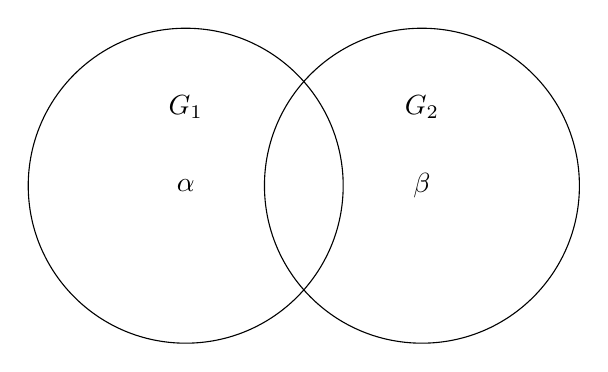
\begin{tikzpicture}
	  \node (A) [draw,circle,minimum size=4cm]  at (0,0) {$\alpha$};
	  \node (G1) [above of=A] {$G_1$};
	  \node [draw,circle,minimum size=4cm] (B) at (0:3cm) {$\beta$};
	  \node (G2) [above of=B] {$G_2$};
	\end{tikzpicture}         
    \end{center}
\caption{Two mutually incompatible grammars}
%\label{grammars}
\end{figure}



\begin{figure}
\begin{center}
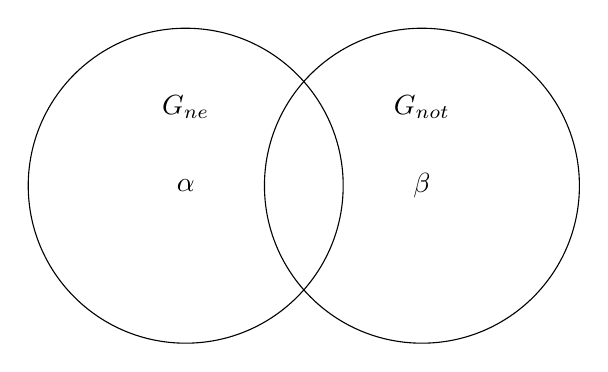
\begin{tikzpicture}
  \tikzset{venn circle/.style={draw,circle,minimum width=#1}}
  \node (A) [venn circle = 4cm]  at (0,0) {$\alpha$};
  \node (G1) [above of=A] {$G_{ne}$};
  \node [venn circle = 4cm] (B) at (0:3cm) {$\beta$};
  \node (G2) [above of=B] {$G_{not}$};
%   \node[below] at (barycentric cs:A=1/2,C=1/2 ) {$G_1 G_2$};   
\end{tikzpicture}       
\end{center}
\caption{Two mutually incompatible grammars}
\label{grammars}
\end{figure}


\begin{figure}
    \begin{center}
        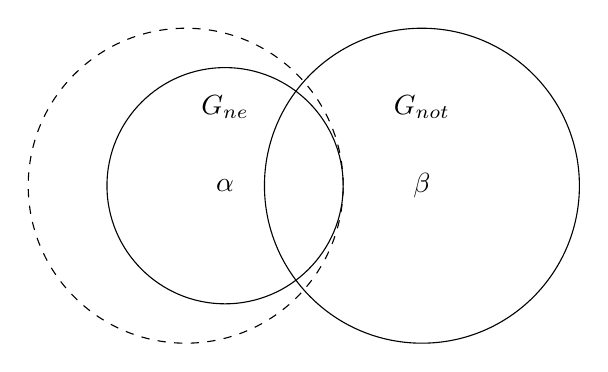
\begin{tikzpicture}
	  \node (A) [draw,circle,dashed,minimum size=4cm]  at (0,0) {};
	  \node [draw,circle,minimum size=3cm] (C) at (0:.5cm) {$\alpha$};
	  \node (G1) [above of=C] {$G_{ne}$};
	  \node [draw,circle,minimum size=4cm] (B) at (0:3cm) {$\beta$};
	  \node (G2) [above of=B] {$G_{not}$};
	\end{tikzpicture}         
    \end{center}
\caption{Two mutually incompatible grammars}
%\label{grammars}
\end{figure}

\begin{figure}
    \begin{center}
        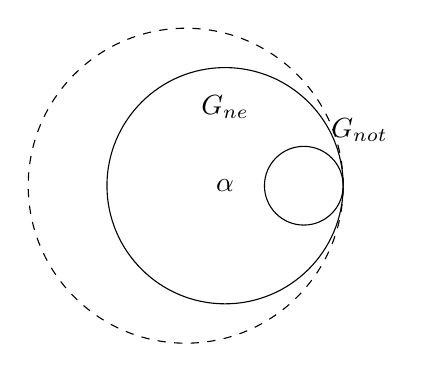
\begin{tikzpicture}
	  \node (A) [draw,circle,dashed,minimum size=4cm]  at (0,0) {};
	  \node [draw,circle,minimum size=3cm] (C) at (0:.5cm) {$\alpha$};
	  \node (G1) [above of=C] {$G_{ne}$};
	  \node [draw,circle,minimum size=1cm] (B) at (0:1.5cm) {};
	  \node (G2) [above right of=B] {$G_{not}$};
	\end{tikzpicture}         
    \end{center}
\caption{Two mutually incompatible grammars}
%\label{grammars}
\end{figure}

\begin{figure}
 \begin{center}
         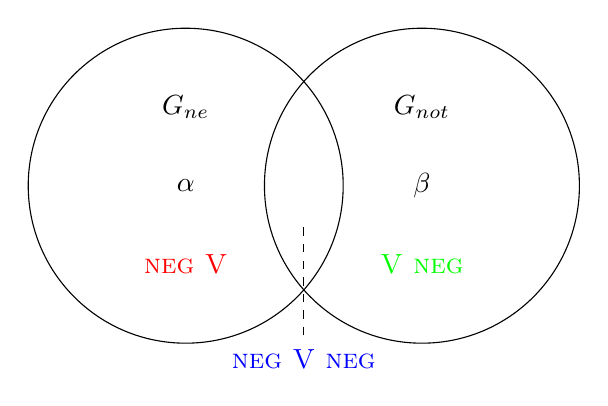
\begin{tikzpicture}
 	  \node (A) [draw,circle,minimum size=4cm]  at (0,0) {$\alpha$};
 	  \node (G1) [above of=A] {$G_{ne}$};
 	  \node [draw,circle,minimum size=4cm] (B) at (0:3cm) {$\beta$};
 	  \node (G2) [above of=B] {$G_{not}$};
    	  \node (alpha) [below of=A] {\textsc{\color{red} neg V}};
    	  \node (neither) at (1.5,-2.2) {\textsc{\color{blue} neg V neg}};	  
   	  \node (beta) [below of=B] {\textsc{\color{green} V neg}};
	  \draw [dashed] (1.5,-1.9) -- (1.5,-.5);
 	\end{tikzpicture}         
     \end{center}
\end{figure}


On the standard version of the model, if $\beta \neq \alpha$, then one grammar or the other will win out. Thus, we would expect that starting from a given point in time an incoming grammar would only spread if it had more initial evidence in favor of it. However, this rests on the assumption that no mechanisms other than acquisition are acting on the distribution of forms. Our analysis thus far suggests that this need not be the case.


\begin{figure}
\begin{center}
 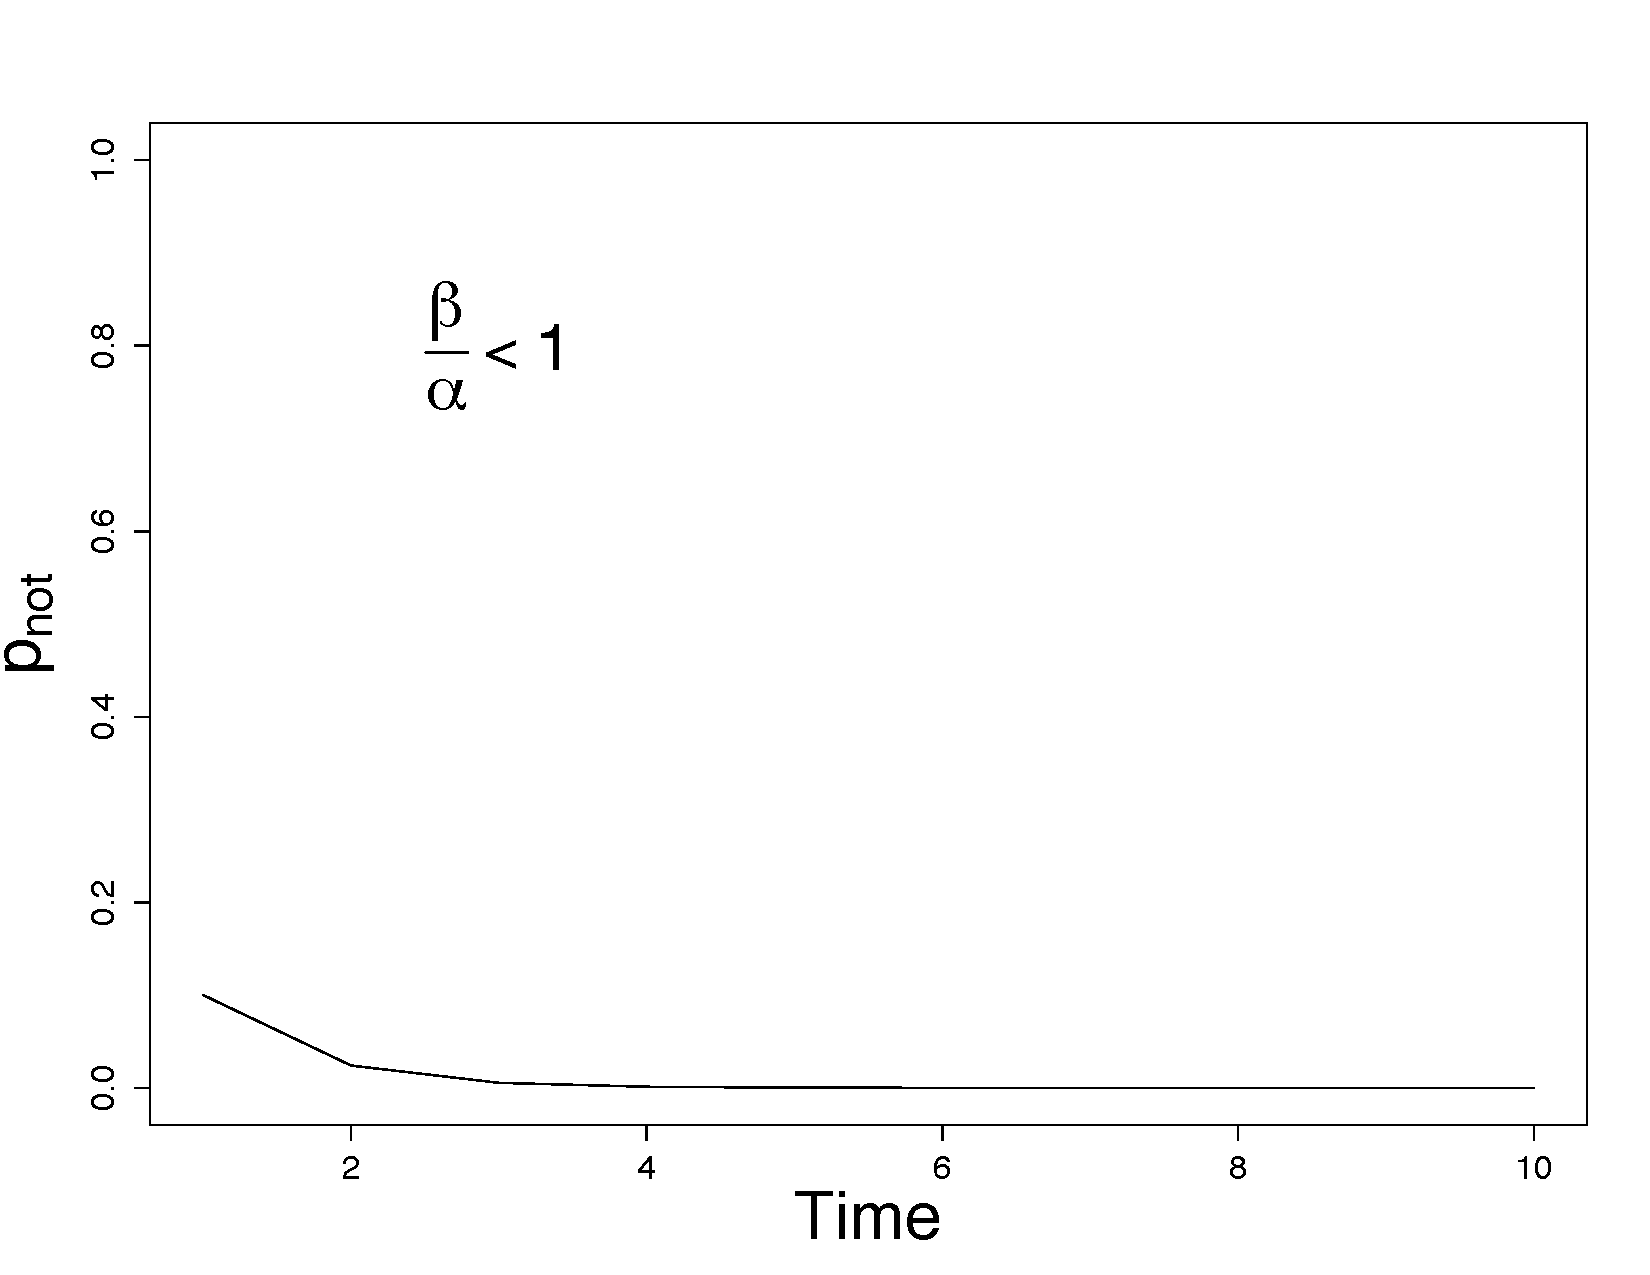
\includegraphics[width=\textwidth]{loss-solution.pdf}\\
\end{center}
	\caption{}
\end{figure}


\begin{figure}
\begin{center}
	 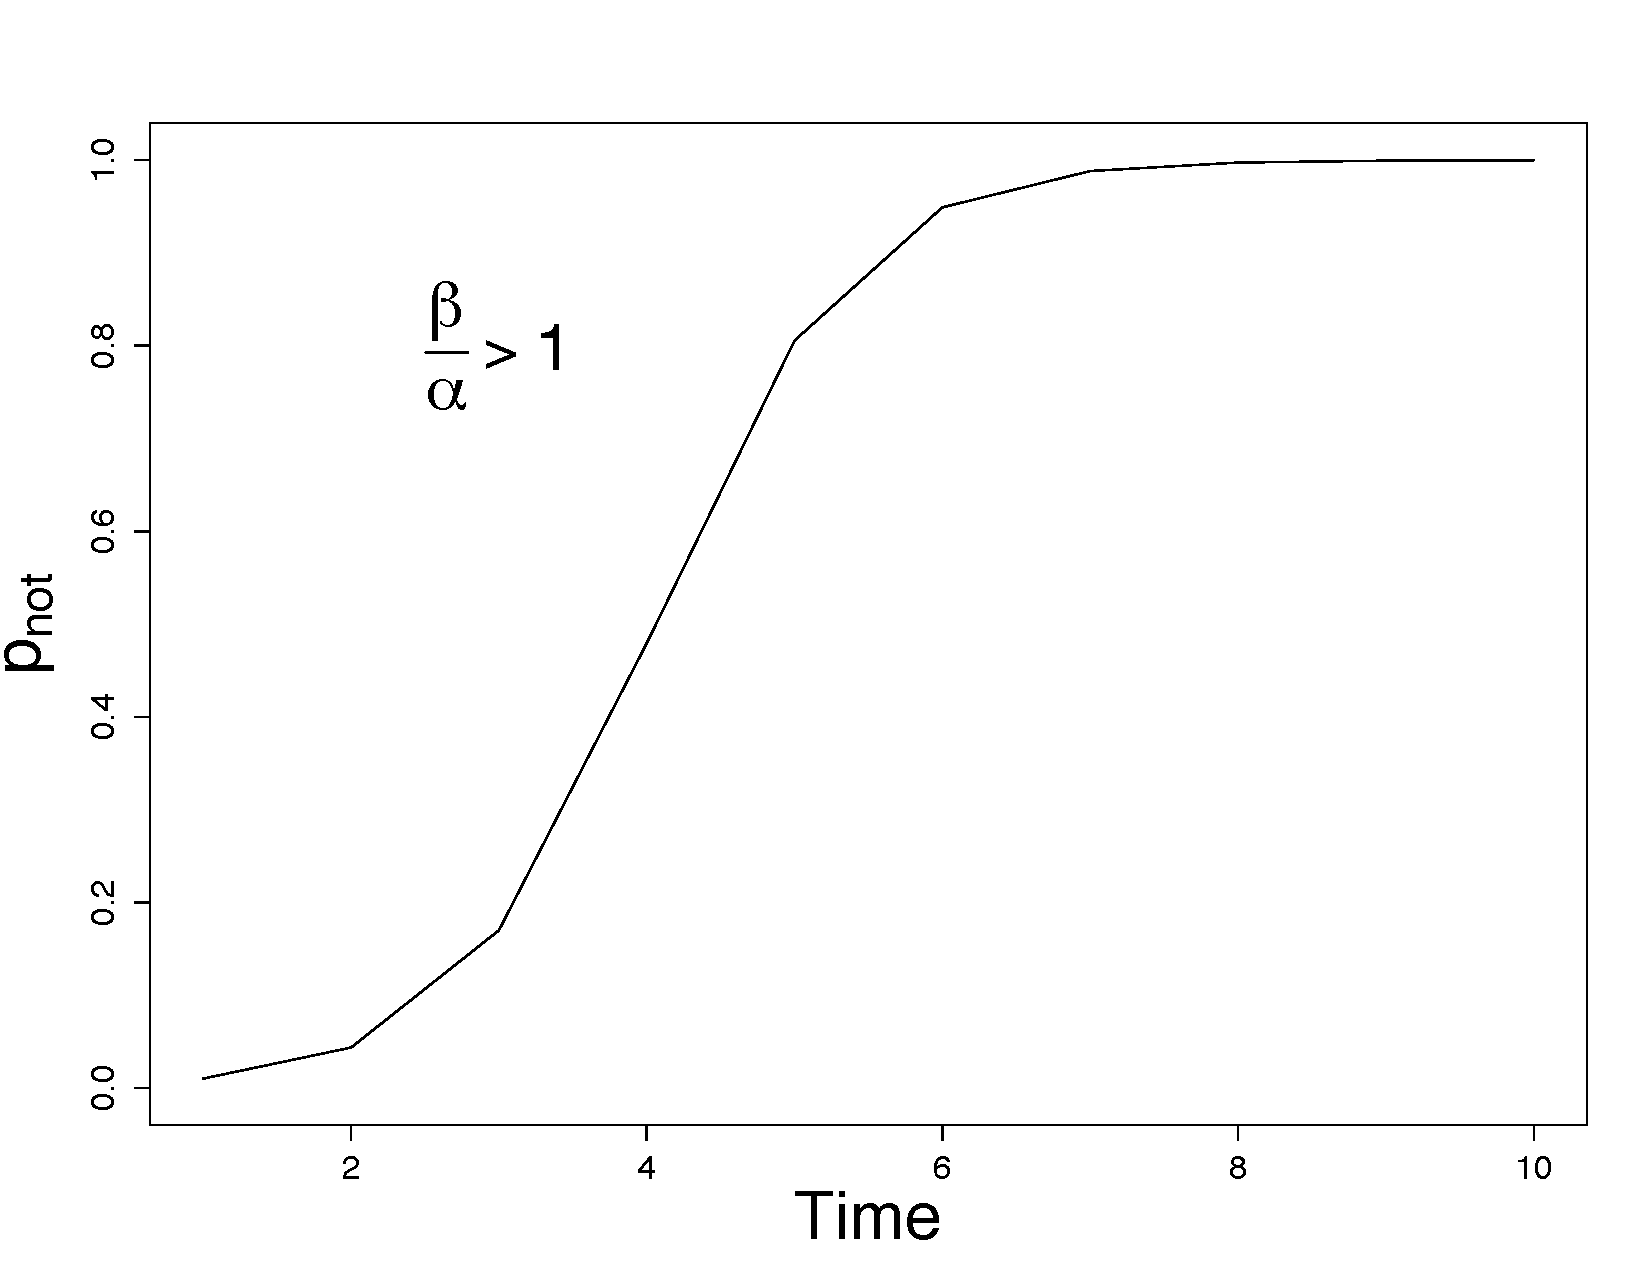
\includegraphics[width=\textwidth]{gain-solution.pdf}\\
\end{center}
	\caption{}
\end{figure}

Here we consider the two mechanisms that might factor into the trajectory of the change. First, the increase of postverbal negation directly impacts the change insofar as it diminishes $\alpha$. Second, there are instances of $ne$ that provide evidence that it does not bear the negative feature, rendering $\beta$ nonzero.  Both mechanisms alone, or in combination can be used to make predictions about the trajectory of the change over time. We consider each mechanism in isolation and then in tandem, determining whether either is sufficient   to cause the change in isolation.


As noted in the previous section, the use of the postverbal negator spreads up to a point, which is determined by the bias of the speaker. At the most, this can result in the reduction of $\alpha$ to $0$. That is, if $ne...not$ is the only form of negation ever used, then there is equal evidence that $ne$ and $not$ express negation. That is, there is no reason why we would expect one form to replace the other. This means that pragmatic pressures are not sufficient in isolation to affect the change. Rather, there must be some precursors that pave the way for the change. This is an interesting, but arguably welcome limitation to the scope of pragmatic pressures. Use can only do so much.  Similarly, unless the evidence is already in favor of $not$ as the expression of negation there is no chance that the change will go through. That is, neither change is sufficient to bring about the change on its own. However, together, the two offer insight into how the change takes place.

We consider how increased use of the postverbal negator might interact independent evidence that $not$ is the expression of negation. Namely, we consider the appearance of all forms in environments that license the appearance of negative polarity items, which are indicative of the lack of the abstract negative feature. These include the scope of negation, certain positions in comparative constructions, antecedents of conditionals (when not expressing actual negation), the restrictor of universal quantifiers, in the scope of verbs of doubting, in embedded clauses under negation, and direct and indirect questions \citep{ladusaw1979, giannakidou1998}. This simply reflects the intuition that NPIs are associated with some negative feature, but not negative in their own right. Occurrence outside these environments can be taken as evidence for the abstract feature. Thus, for both the preverbal and postverbal negators, the amount of evidence that they bear the abstract feature can easily be found for at least some 
of these categories from a corpus. \cite{wallage2008} gives occurrences of the various forms of negation from the Penn-Helsinki Parsed Corpus of Middle English (PPCME2) \citep{ppcme2}  in main clauses, subordinate clauses, \emph{if}-clauses, and in the scope of negation.

\begin{table}[ht]
\begin{center}
\begin{tabular}{@{}cccccccc@{}}
\hline
Main Clauses & & & &Subordinate Clauses &  &   &\\
\hline
Period & \emph{ne} & \emph{ne...not} & \emph{not} & Period & \emph{ne} & \emph{ne...not} & \emph{not}\\
\hline
1150-1250 & 91 & 152 & 3  & 1150-1250 & 279 & 112 & 4  \\
1250-1350 & 48 & 329 & 48  & 1250-1350 & 87 & 147 & 15  \\
1350-1420 & 3 & 108 & 935  & 1350-1420 & 17 & 115 & 905  \\
1420-1500 & 1 & 12 & 928  & 1420-1500 & 7 & 4 & 821  \\
\hline
\end{tabular}
  \caption{Frequency of forms in main and subordinate clauses from}
\end{center}
\end{table}

\begin{table}[ht]
\begin{center}
\begin{tabular}{@{}cccccccc@{}}
\hline
\emph{if}-clauses & & & &In scope of negation &   &   &\\
\hline
Period & \emph{ne} & \emph{ne...not} & \emph{not} & Period & \emph{ne} & \emph{ne...not} & \emph{not}\\
\hline
1150-1250 & 33 & 10 & 0  & 1150-1250 & 33 & 3 & 0  \\
1250-1350 & 12 & 8 & 3  & 1250-1350 & 19 & 6 & 2  \\
1350-1420 & 9 & 5 & 64  & 1350-1420 & 14 & 8 & 55  \\
1420-1500 & 2 & 1 & 51  & 1420-1500 & 4 & 1 & 43  \\
\hline
\end{tabular}
  \caption{Frequency of forms in \emph{if}-clauses and In scope of negation}
\end{center}
\end{table}

Taken together, we can estimate the amount of evidence over time for and against the two grammars. That is, those occurrences of a particular form by itself in a main or a subordinate clause constitute positive evidence for its respective grammar, whereas those occurrences of a particular form in the scope of negation constitute positive evidence for the other grammar. It is not clear whether all the instances of negation in the antecedent of conditionals express negation, so here we leave them out of our counts. The change in the relative evidence across time can be seen in Table \ref{evidence}. 

\begin{table}[ht]
\begin{center}
\begin{tabular}{@{}cccccc@{}}
\hline
Period & $\alpha$ & $\beta$ & $\frac{\beta}{\alpha}$ & \emph{ne...not}\\
\hline
1150-1250 & 370 & 40  & .108 & 277\\
1250-1350 & 137 & 65 & .474 & 490\\
1350-1420 & 75 & 1799 & 23.986 & 236\\
1420-1500 & 51 & 1704 & 33.411 & 18\\
\hline
\end{tabular}
  \caption{Relative evidence for grammars}
\label{evidence}
\end{center}
\end{table}

At some point during the transition from the second to the third period there is a clear tipping point in the amount of evidence for the two grammars. $ne$ goes from being favored as the host of the negative feature to being grossly disfavored. Note that this transition coincides with the peak usage of \emph{ne...not}, suggesting that the increasing use of postverbal negation continued up until a certain point, rendering $not$ the uncontested expression of negation. Both use and acquisition play there parts in bringing about the change.

Now, while this evidence is suggestive, it still leaves the appearance of $not$ by itself a mystery. This follows from the fact that the variational model is not a model of actuation itself. To see this note that the grammar must already be in existence for it to grow. That is, if $q_0 = 0$ then $q_1=0$.

\begin{equation}
     \frac{q_1}{p_1} = \left( \frac{\beta}{\alpha} \right)\frac{q_0}{p_0}
\end{equation}
One possible way of making sense of this actuation stems from the phonetic weight of the preverbal negator. That is, as the postverbal negator increases in frequency, even a small probability of misperceiving the preverbal negator as absent provides evidence for the change, and, importantly, the ultimate loss of the preverbal negator. It might be possible to infer the impact of these misperceptions over time given the predicted dynamics of the learning model. That is, the proportion of a given grammar must exceed a threshold to keep from being effectively washed out by one generation. We can test how a small error rate in misperceptions might counteract this force, and, along with the steady increase in postverbal negation, bring about the eventual loss of the preverbal negator. 